\documentclass[energies,article,submit,moreauthors]{Definitions/mdpi}












\firstpage{1}
\makeatletter
\setcounter{page}{\@firstpage}
\makeatother
\pubvolume{19}
\issuenum{21}
\articlenumber{5024}
\pubyear{2026}
\copyrightyear{2026}
\externaleditor{}
\datereceived{27 September 2026}
\daterevised{16 October 2026}
\dateaccepted{17 October 2026}
\datepublished{22 October 2026}

\Title{Phase-Informed
 ECMS with Soft SOC Safeguarding for a Virtual Hybrid Agricultural Tractor}
\newcommand{\orcidauthorA}{0009-0005-1928-6218}
\Author{Chenyu
 Cui\orcidA{}, Peng Wang and Yucheng Zhang *}
\AuthorNames{Chenyu Cui, Peng Wang and Yucheng Zhang}
\address[1]{Prospective Research Laboratory, Institute of Computing Technology, Chinese Academy of Sciences, \mbox{Beijing 100190,} China; cuichenyu25s@ict.ac.cn (C.C.); wangpeng2021@ict.ac.cn (P.W.)
}

\corres{\hangafter=1 \hangindent=1.05em \hspace{-0.82em} Correspondence: zhangyucheng@ict.ac.cn}

\abstract{Fuel reductions can be confounded by battery depletion or unreported control corrections. This theoretical study examines phase-informed equivalent-consumption minimization (ECMS) with a soft state-of-charge (SOC) safeguard in an ideal power-split virtual tractor. The model includes planetary kinematics, machine limits, battery resistance and engine execution constraints. Numerical conservation checks verify implementation without providing empirical validation. The frozen adaptive configuration reproduces the submitted 5.676\% normalized fuel saving. On 20 independent paths, it achieves 5.951\% saving relative to matched load following, with all paths meeting a $10^{-4}$ terminal-SOC tolerance. Removing the safeguard leaves no terminal-valid paths. Removing adaptation instead gives 7.091\% saving with the same safeguard, while increasing mean interventions from 94.8 to 150.5. Adaptation therefore changes the fuel--intervention trade-off rather than improving fuel economy. Same-parameter cycle, capacity and map audits retain positive valid-pair savings but expose terminal failures and an empty-action demand boundary. A historical approximately 20\% full-information diagnostic is reported separately under a favorable map, different electrical limits and relaxed terminal band. The contribution is an auditable comparison of fuel, terminal charge and corrections within a declared virtual platform, without recursive-feasibility guarantees or field-economy predictions.}
\keyword{hybrid agricultural tractor; energy management; ECMS; state of charge; soft safeguard; ablation; virtual powertrain; theoretical simulation}
\begin{document}

\section{Introduction}
Agricultural traction demand changes with implement draft, soil resistance, grade and task phase. Electrification can buffer this demand, but~the resulting fuel benefit depends on the architecture, component characteristics and energy-accounting convention. Studies of solar-assisted plug-in tractors, parallel hybrid tractors and predictive tractor energy management illustrate this diversity~\cite{mousazadeh2011,mocera2020,curiel2023}. Differences in engine rated power and loading also affect tractor fuel use~\cite{jilek2008,janulevicius2010}. Consequently, a~percentage obtained on one short virtual task is not a transferable field-economy~estimate.

Two comparison difficulties motivate this work. First, an~online strategy can apparently reduce fuel by ending with less battery energy. Second, a~feasibility correction can alter the applied command substantially while remaining absent from the reported policy description. These effects should be distinguished from economic improvement. This requires common initial conditions and component limits, an~explicit terminal-SOC criterion, matched same-seed baselines and separate counts of completed, terminal-valid and failed trajectories. Energy normalization is useful for diagnosing residual battery imbalance, but~does not turn an inadmissible trajectory into a successful charge-sustaining~result.

ECMS is attractive because it selects the current operating point using a fuel-equivalent battery-energy cost~\cite{musardo2005}. SOC feedback, a~task-phase reference and a finite-action safeguard can then serve different purposes: economic load shifting, guidance toward the terminal charge target and correction of a proposal that conflicts with that guidance. Combining these mechanisms does not establish which one causes a gain. In~particular, an~adaptive factor may reduce correction frequency while worsening fuel economy relative to a fixed factor subject to the same safeguard. The~present revision explicitly tests that~possibility.

This study asks whether the submitted adaptive configuration remains charge-sustaining on independent synthetic tasks, which modules account for its fuel--charge trade-off, and~how its conclusions depend on the virtual model. The~scope is an ideal power-split architecture with researcher-defined component inputs. The~architecture is physically constrained and numerically checked, but~it is not identified from a tractor, an~engine bench or a battery pack. This distinction separates verification of the equations and software from validation against a physical system~\cite{sargent2013}.

The article makes three contributions. First, it specifies the applied control chain and its two different empty-set branches: a hard-feasible action set that may be empty, and~a soft SOC corridor that may be relaxed. Second, it adds independent, same-platform ECMS comparisons and module ablations that report favorable and unfavorable outcomes together. Third, it corrects the battery formulation and the frozen-parameter audit, and~organizes controller performance, mechanism sensitivities and full-information diagnostics into separate evidence categories. The~contribution is this integration and attribution within a reproducible virtual experiment; ECMS adaptation, SOC feedback and finite-action filtering are not individually claimed as new~algorithms.

\section{Related Work and Study~Positioning}
Tractor hybridization has been examined through parallel-architecture analysis and model-based hardware-in-the-loop development~\cite{mocera2020,mocera2020b}, MPC-based energy management~\cite{curiel2023}, reinforcement-learning control~\cite{wu2024}, and~fuel-cell hybridization~\cite{zhao2024,zhang2024freq}. Recent agricultural-tractor studies also report dynamic-programming energy management for OS-ECVT and series-hybrid architectures~\cite{zhang2024osecvt,yan2024series}, while system-level work has examined optimal series-hybrid powertrain design~\cite{perez2024}. These studies differ in powertrain architecture and validation level. In~particular, a~hardware-in-the-loop investigation informed by field characterization is a different evidence class from the synthetic virtual experiments reported here. We do not rank these published controllers using their reported~percentages.

The wider hybrid-vehicle literature distinguishes full-trajectory offline optimization~\cite{xie2016}, adaptive ECMS~\cite{musardo2005} and~predictive control using different information sets~\mbox{\cite{ripaccioli2010,zhang2017,wang2016}}. Recent fuel-cell and hybrid-tractor studies further show that component sizing and power-allocation choices are coupled: optimal sizing has been evaluated with unit-mileage-cost objectives~\cite{wang2025sizing}, whereas the present paper holds the virtual platform fixed and studies controller attribution. Predictive diesel management can additionally account for transient engine behavior~\cite{huo2018}. Our engine model instead uses steady conversion efficiency with a running-power ramp and prescribed start logic; it cannot reproduce turbocharger dynamics or transient emissions. Equivalent-circuit battery models support computationally tractable state estimation and energy accounting~\cite{plett2004}, but~omitting polarization and temperature dynamics limits the interpretation of a pack-level virtual~result.

Predictive safety-filter research establishes stronger constraint guarantees through explicit predictive constructions and their assumptions~\cite{wabersich2021}. Our successor-SOC corridor has neither a robust invariant set nor a backup policy proven feasible under all future admissible loads. We therefore replace the previous ``viability-shield'' terminology with ``soft SOC safeguard.'' The method keeps current hard constraints intact and makes its corrections observable; observed terminal success is an experiment outcome, not a mathematical~guarantee.

Relative to conventional ECMS, the~question is whether public task-phase guidance and an internal successor-SOC filter change the attainable balance between fuel, terminal SOC and correction frequency under the same discrete plant. This is tested directly against fixed and adaptive ECMS, including fixed ECMS with the identical safeguard. The~earlier MPC investigations are retained in Supplementary Material S7 as conditional negative controls. They use a different legacy implementation and are not treated as same-plant competitors to the revised primary~experiment.

\section{Materials and~Methods}
\unskip
\subsection{Ideal Power-Split Plant and Its~Boundary}
The required wheel-side demand is defined by
\begin{equation}\label{eq:demand}
 P_w=\max\!\left(0,\frac{(K_sF_d+F_r+m_vgq)v}{\eta_t}\right),
\end{equation}
where $q$ is the prescribed grade input, $F_r=2500$ N, $m_v$ = 18,000 kg and $\eta_t=0.88$. The~nonnegative demand construction does not model braking-energy recovery. Acceleration and longitudinal speed tracking are not simulated; speed and draft are task inputs. An~18 kW accessory load is added on the electrical bus and is not folded into $P_w$.

The engine is connected to an ideal carrier, MG1 to the sun branch and the wheel drive to the ring branch; MG2 supplies the remaining wheel-side power. With~ring-to-sun tooth ratio $\kappa=2.6$, final-drive ratio $i_f=60$ and wheel radius $r_w=0.94$ m, the~implemented relations are
\begin{align}
 n_r&=\frac{60v i_f}{2\pi r_w},&
 n_s&=(1+\kappa)n_e-\kappa n_r,\label{eq:kinematics}\\
 P_r&=P_e\frac{\kappa}{1+\kappa}\frac{n_r}{n_e},&
 P_1&=P_e-P_r,& P_2&=P_w-P_r.\label{eq:split}
\end{align}
When

 the engine is off, $P_e=P_r=P_1=0$ and $n_s=-\kappa n_r$. Positive $P_1$ denotes the mechanical power available to MG1 for generation, whereas positive $P_2$ denotes MG2 motoring. Equation~(\ref{eq:split}) can represent circulating power; it does not require $P_r/P_e$ to remain below one. Candidate machine power and speed limits reject inadmissible points. Gear losses, shaft inertia, a~calibrated tooth geometry and clutch dynamics are absent. The~architecture is therefore an ideal power-split representation, not a calibrated OS-ECVT product model. Independent torque envelopes are also absent; power and speed checks do not substitute for low-speed torque~validation.

For a mechanical machine input $P$ positive in motoring convention, define
\begin{equation}
 \mathcal{E}(P)=\begin{cases}P/\eta_m(P),&P\geq0,\\P\eta_m(P),&P<0.\end{cases}
 \qquad P_b=\mathcal{E}(P_2)+\mathcal{E}(-P_1)+P_{aux}.
\end{equation}
The implemented motor map is power-dependent, although~the function accepts a speed argument. It is not a calibrated two-dimensional speed--torque map. Its analytic expression and the complete fixed inputs are given in Supplementary Material S1. This simplification keeps conversion losses visible while avoiding unsupported machine-specific~claims.

\subsection{Battery, Fuel Map and Parameter~Representativeness}
The battery uses an OCV--resistance algebraic model with positive current denoting discharge:
\begin{align}
 V_{oc}(s)&=650+80(s-0.55)\ \mathrm{V},&R_b&=0.045\ \Omega,\\
 D&=V_{oc}^2-4R_bP_b,& I_b&=\frac{V_{oc}-\sqrt{D}}{2R_b},\label{eq:battery}\\
 V_t&=V_{oc}-R_bI_b,&
 s_{k+1}&=s_k-\frac{I_b\Delta t}{3600Q_{Ah}},\quad Q_{Ah}=\frac{E_{Wh}}{650}.
 \label{eq:soc}
\end{align}
Equation~(\ref{eq:soc}) corrects the energy-based expression in the submitted manuscript and matches the implemented coulomb counting. Power is related to terminal voltage by $P_b=V_tI_b$, and~ohmic loss is $R_bI_b^2$. Candidates require $D\geq0$, $|P_b|\leq180$ kW and $s_{k+1}\in[0.20,0.80]$. No separate pack-current, terminal-voltage, thermal or aging limits are imposed. Reported current is diagnostic, not a validated pack safety rating. The~model has no RC polarization state, so we do not call it a first-order dynamic equivalent~circuit.

The primary engine map uses the speed--load dependence of the published Deutz BF 6M 2012 C consumption regression~\cite{devyanin2023}; the regression is normalized and its efficiency is rescaled and capped at 0.42 for a declared 300 kW virtual engine (Table~\ref{tab:parameters}). Its exact transform, guard values and clipping are documented in S1. Rescaling preserves a reference trend but neither the source engine's absolute fuel consumption nor a measured 300 kW torque envelope. The~value 0.42 corresponds to approximately 200.74 g/kWh at the declared lower heating value of 42.7 MJ/kg; this dimensional conversion is a consistency check, not evidence that the target engine achieves that efficiency. Figure~\ref{fig:maps} shows the map actually used, rather than an illustrative unconnected~map.

\begin{table}[H]
\caption{Primary
 virtual-platform choices and their interpretation. All numerical values are researcher-defined inputs, except~the cited engine-regression shape; none is a measured target-platform~rating.}\label{tab:parameters}
\small\begin{tabularx}{\linewidth}{@{}p{.24\linewidth}p{.22\linewidth}X@{}}\toprule
\textbf{Quantity} & \textbf{Primary Value} &\textbf{Reason and Limitation} \\\midrule
Engine power; stable floor & 300; 60 kW & Nominal power scale; positive candidates begin at 20\% rating. \\
Running ramp; start rule & 40 kW/s; start at 60 kW & Explicit virtual actuator restrictions; start is a discrete transition, not a measured~transient. \\
Machine and bus limits & 180 kW each & Electrical-to-engine power ratio 0.60; common to primary~comparisons. \\
Battery energy; voltage & 200 kWh; 650 V & 307.69 Ah; 0.667 rated-engine hours. This large store favors buffering and is not packaging~validation. \\
Battery resistance & 0.045 $\Omega$ & Prescribed ohmic loss; no temperature or polarization~dynamics. \\
Machine speeds & $|n_1|,|n_2|\leq7000$ rpm & Proxy operating envelope; no independent torque~curve. \\
Task/sampling/grid & 600 s/1 s/5 kW & Finite enumerated operating points; grid sensitivity is reported~separately. \\
SOC tolerance & $10^{-4}$ & Strict revised evaluation; no post-run SOC repair. \\\bottomrule
\end{tabularx}
\end{table}

These scales are sufficient to define a reproducible virtual experiment, but~not to establish physical representativeness for a tractor. We test the chosen battery scale at 120 and 280 kWh, the~action grid at 10 and 2.5 kW, and~explicitly different low-load map shapes. These perturbations address selected sensitivities, not all combinations of component uncertainty. The~historical 150 kW platform is confined to legacy diagnostics; the revised primary comparisons all use 180~kW.

\begin{figure}[H]
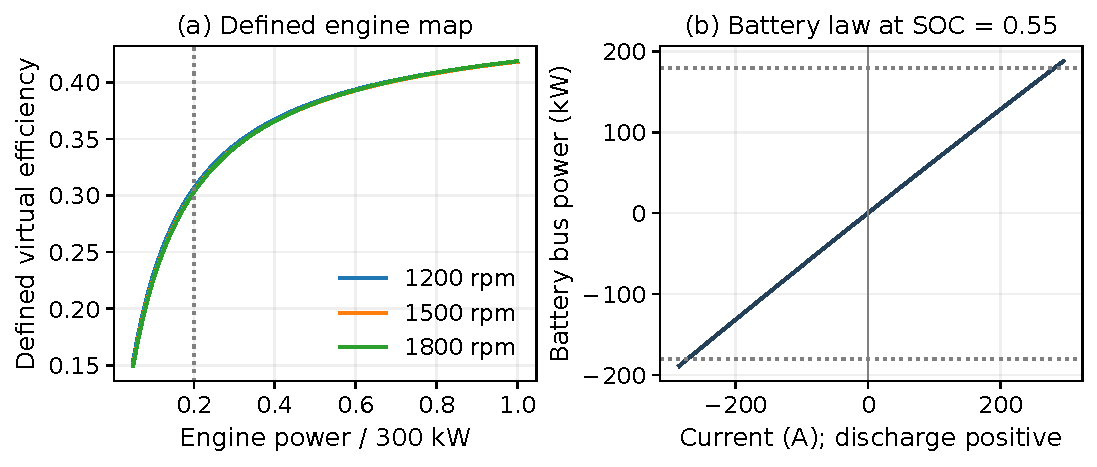
\includegraphics[width=\linewidth]{figures/revision_model_maps.pdf}
\caption{Implemented primary virtual inputs: (\textbf{a}) rescaled literature-shaped engine efficiency at the three candidate speeds; (\textbf{b}) OCV--resistance battery law at the target SOC. The~motor map is specified analytically in S1. These are defined model inputs, not calibration~results.}\label{fig:maps}
\end{figure}
\unskip

\subsection{Causal ECMS and the Soft SOC~Safeguard}
The controller state is $x_k=(s_k,P_{e,k-1},n_{e,k-1},t_{on,k},t_{off,k})$. Information available at decision $k$ comprises this state, the~present demand and speed, the~public task time and declared task duration $N\Delta t$. No evaluated-seed future disturbance is accessed. Engine-speed candidates are 1200, 1500 and 1800 rpm. Positive powers lie on the 5 kW grid from 60 to 300 kW. A~running engine can change power by at most 40 kW per 1 s step, can stop only after 5 s on, and~can restart only after at least 1 s off. Cold start enters the 60 kW point; shutdown and start are discrete transitions, not subject to the continuous running-ramp~bound.

Let $\mathcal{F}_k$ contain the candidates satisfying these execution restrictions, planetary relations, machine limits, battery discriminant, bus-power limit and successor physical SOC bounds under the current demand. If~an electric-only candidate requires $|P_b|>rP_b^{max}$, $r=0.65$, and~an engine-on feasible candidate exists, the~conditional reserve rule retains the engine-on candidates as $\mathcal{F}^r_k$. Otherwise, $\mathcal{F}^r_k=\mathcal{F}_k$. The~117 kW trigger discourages electric-only operation near the bus limit; it does not reserve 35\% headroom for every candidate or guarantee accommodation of the next unknown load. Start and dwell remain common execution constraints, not claimed innovations of~ECMS.

The economic proposal minimizes
\begin{align}
 J_k(a)&=m_{f,k}(a)+\lambda_k\frac{P_{b,k}(a)\Delta t}{H_f\eta_{eq}}1000
       +w_Q\frac{|P_{b,k}(a)|\Delta t}{3.6\times10^6}+w_{sw}z_k(a),\label{eq:score}\\
 \lambda_k&=\max\{0.05,\lambda_0+K_p(s_k^{ref}-s_k)\},\qquad
 a_k^0\in\arg\min_{a\in\mathcal{F}^r_k}J_k(a).
\end{align}
Fuel mass $m_f$ is in grams and includes 2 g on engine start. $H_f$ is in J/kg, $\eta_{eq}=0.40$, $w_Q=0.02$ g/kWh and $w_{sw}=0.2$ g. The~indicator $z_k$ is one for either an on-to-off or off-to-on transition, correcting the submitted description of an exclusively start-related switching penalty. Integral SOC feedback is disabled ($K_i=0$). Negative battery power produces a charging credit in the equivalent-energy term; throughput is penalized by its absolute~value.

The public reference follows a 270 s task schedule: 0.565 SOC for 0--120 s, linear decline to 0.545 for 120--240 s and return to 0.55 for 240--270 s. The~reference offset is attenuated during the final 270--120 s and becomes 0.55 for the last 120 s. This is a chosen energy-buffer schedule aligned with public task phases, not an optimized reference computed from future realized demand. The~complete piecewise rule appears in~S2.

For the successor at step $k$, let $\rho_k=\max\{0,(N-k-1)/(N-1)\}$ and $b_k=b_0\rho_k^2$, $b_0=0.045$. The~soft successor-SOC set is
\begin{equation}
 \mathcal{G}_k=\{a\in\mathcal{F}^r_k:\ |s_{k+1}(a)-s_k^{ref}|\leq b_k\}.
\end{equation}
If $\mathcal{G}_k$ is nonempty, the~minimum-cost candidate in it is applied. If~it is empty but $\mathcal{F}^r_k$ is nonempty, the~controller minimizes $|s_{k+1}-s_k^{ref}|$ first and $J_k$ second. Hard constraints are preserved and only the soft reference criterion is relaxed. If~$\mathcal{F}_k$ is empty, the~virtual trajectory terminates with a recorded failure; no least-violating command is applied. Figure~\ref{fig:architecture} gives the implemented~order.

\begin{figure}[H]
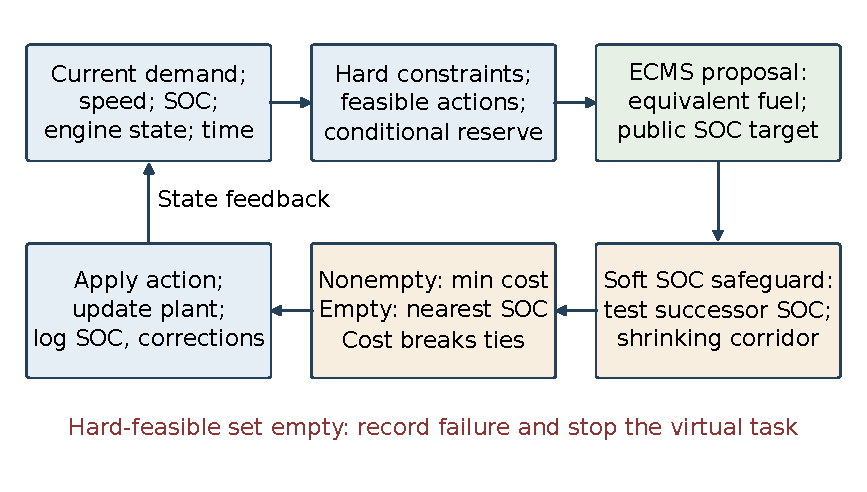
\includegraphics[width=\linewidth]{figures/revision_architecture.pdf}
\caption{Applied causal chain. Physical candidate generation precedes the economic proposal. A~soft-corridor empty set and a hard-feasible empty set lead to different branches. No experiment-runner terminal correction is~added.}\label{fig:architecture}
\end{figure}

An intervention means that the applied action differs from $a_k^0$. A~soft-corridor empty event is recorded separately and need not imply an intervention if the nearest-SOC action equals $a_k^0$. At~the last sample, $b_k=0$, so a discrete candidate commonly cannot hit the reference exactly; terminal success is assessed by $|s_N-s_0|\leq10^{-4}$ after simulation. The~corridor is not a backward-reachable or invariant set. Current constraint satisfaction does not ensure $\mathcal{F}_{k+1}\ne\emptyset$, and~narrowing $b_k$ does not prove terminal closure. These limitations are part of the controller definition, not exceptions added after a failed~experiment.

\subsection{Numerical Verification and Experimental~Protocol}
We sampled 1200 virtual states and current-demand points using seed 5240 and checked all state-consistent candidates. Of~42,084 actions, 28,093 were feasible. On~feasible actions, the maximum mechanical power-balance residual was $5.82\times10^{-11}$ W and the maximum battery-power residual was $7.42\times10^{-10}$ W. Planetary kinematics, bus summation and SOC-update residuals were zero at reported precision. At~$s=0.55$ and $P_b=\pm180$ kW, discharge current was 282.45 A and charge current was $-271.81$ A, with~respective ohmic losses 3.590 and 3.325 kW. These checks verify algebra and numerical implementation~\cite{sargent2013}; they do not validate parameter values against~hardware.

Applied-command checks additionally cover 60 independent adaptive, shared-safeguard fixed and baseline trajectories (36,000 samples), with~no cold-start, running-ramp, dwell, bus or physical-SOC violations. These finite execution checks likewise provide no recursive-feasibility theorem (S1).

The primary synthetic work cycle repeats idle (30 s), transport (90 s), ploughing (120 s) and turn (30 s), with~5 s transitions. Correlated soil and grade disturbances are generated independently of the controller. The~task-generation equations and seed ledger are in S3. The~submitted development seeds 3100--3105 selected $(\lambda_0,K_p,b_0)=(1,40,0.045)$ from 75~candidates. Selection required six terminal-valid paths, preferred mean interventions no greater than 100 and then maximized development saving. The~submitted holdout seeds 3120--3139 are replayed without selecting another parameter. The~revised independent set is 5120--5139. All new primary tests and sensitivities retain $K_p=40$; previously reported $K_p=60$ cross-cycle audits are historical, separately labeled~data.

The matched load-following baseline shares the plant, initial SOC 0.55, candidate restrictions and public reference. It chooses an internally charge-restoring action by matching a reference battery power; it is not an unconstrained engine-only tractor. The~submitted baseline used an internal band computed with the default  0.001 setting, although~its terminal errors meet $10^{-4}$. New comparisons instead use an explicit $10^{-4}$ baseline setting; exact submitted replay/attribution retains the recorded submitted baseline. Differences between those protocols are not interpreted as controller improvement. Fixed and adaptive conventional ECMS additionally receive equal 15-candidate development budgets on new seeds 5100--5105, then are frozen before 5120--5139. A~fixed ECMS arm uses the same phase reference, reserve and SOC safeguard as the primary adaptive arm. This isolates adaptation without handicapping its comparator with the absence of terminal guidance. Candidate ranges, selection rules, all candidates and the baseline equation are in~S2--S4.

Frozen one-module-removal tests disable adaptation, phase reference, SOC filtering or reserve separately. A~stepwise sequence additionally adds phase guidance, reserve and finally the SOC filter to conventional adaptive ECMS while keeping $\lambda_0=1$, $K_p=40$. These are conditional ablations, not additive allocations of the 5.676\% saving: modules interact through state trajectories and feasible sets. Cold start and dwell constraints are not removed in the primary comparison because doing so changes the allowed actuator~behavior.

Every trajectory is classified as (i) completed and terminal-valid, (ii) completed but terminal-invalid, or~(iii) hard-action failure. Strict-valid paired savings require both the controller and same-seed baseline to complete and meet $10^{-4}$. No failed or SOC-invalid trajectory enters that statistic. All counts are retained, including failures of the baseline. Define
\begin{equation}
 m_f^{norm}=m_f+\frac{(s_0-s_N)E_{Wh}\,3600}{H_f\eta_{norm}}1000,
 \qquad \eta_{norm}=0.42,
\end{equation}
and $S=100(m_{f,B}^{norm}-m_{f,C}^{norm})/m_{f,B}^{norm}$. Fuel volume uses 832 g/L. The~distinction between $\eta_{eq}=0.40$ in control and $\eta_{norm}=0.42$ in reporting is intentional. The~SOC-to-energy term uses nominal capacity, not integration of state-dependent OCV. Normalization is diagnostic accounting, not an appended physical recharge, and~strict SOC acceptance remains independent of it. Completed-only normalized means are labeled diagnostic when terminal validity fails. Student-$t$ intervals describe variability of paired savings across the declared generator seeds; they are not confidence intervals for a physical tractor population. Results from different valid subsets are not direct controller~rankings.

\section{Results}
\unskip
\subsection{Submitted Replay and Independent Frozen~Test}
The submitted 20 strict-audit fuel trajectories reproduce to a maximum difference of less than $10^{-10}$ L. Their normalized mean remains 5.676\%, with~the original $5.52\times10^{-5}$ maximum terminal SOC error. The~additional frozen adaptive test gives 5.951\% normalized saving (95\% interval 5.352--6.549\%) and 5.951\% raw saving on 20/20 valid same-seed pairs. The~maximum terminal SOC error is $1.88\times10^{-6}$; mean interventions, soft-empty events and starts are 94.8, 62.5 and 7.2 per 600 s trajectory, respectively. This replicates the saving direction within the declared generator and virtual model, without~replacing the original 5.676\% result or implying that the extra digits are field~precision.

\subsection{Ablations and Conventional ECMS~Comparisons}
Table~\ref{tab:ablation} and Figure~\ref{fig:ablation} separate the outcomes of each removed module. The~SOC filter accounts for the strongest difference in terminal validity: removing it leaves 0/20 terminal-valid paths despite completion of all paths. Removing phase guidance retains only 16/20 valid paths and has a maximum SOC residual 0.00432. Its 8.786\% valid-pair saving is conditional on those 16 pairs and cannot be ranked against a 20-pair result without acknowledging the selection~difference.

\begin{table}[H]
\caption{Frozen one-module removals on independent seeds 5120--5139. All 20 paths complete for each row. Savings and intervals use only terminal-valid baseline/controller pairs; SOC maxima and intervention means use all completed~paths.}\label{tab:ablation}
\small\begin{tabularx}{\linewidth}{@{}Xrrrr@{}}\toprule
\textbf{Variant} & \textbf{Valid Pairs} & \textbf{Saving (\%)} & \textbf{Max \boldmath$|\Delta s|$} & \textbf{Interventions} \\\midrule
Frozen adaptive + safeguard & 20/20 & 5.951 & $1.88\times10^{-6}$ & 94.8 \\
Fixed factor + same safeguard & 20/20 & 7.091 & $2.07\times10^{-6}$ & 150.5 \\
Without public phase & 16/20 & 8.786 & $4.32\times10^{-3}$ & 60.1 \\
Without SOC safeguard & 0/20 & -- & $6.27\times10^{-3}$ & 0 \\
Without electric reserve & 20/20 & 5.958 & $1.69\times10^{-6}$ & 93.1 \\\bottomrule
\end{tabularx}
\end{table}

Removing adaptation gives 7.091\% saving (95\% interval 6.025--8.157\%) with all 20 pairs valid. On~the same seeds, the~adaptive arm's saving is 1.140 percentage points lower. Its mean interventions are 37.0\% fewer, but~its mean starts are 7.2 rather than 6.9. Thus, fewer interventions do not imply fewer starts or better fuel economy. Removing reserve changes mean saving by only 0.007 percentage points here and increases starts to 7.65. The~reserve rule is a declared instantaneous operating preference; this test does not establish robustness to larger future demand~jumps.
\vspace{-6pt}
\begin{figure}[H]
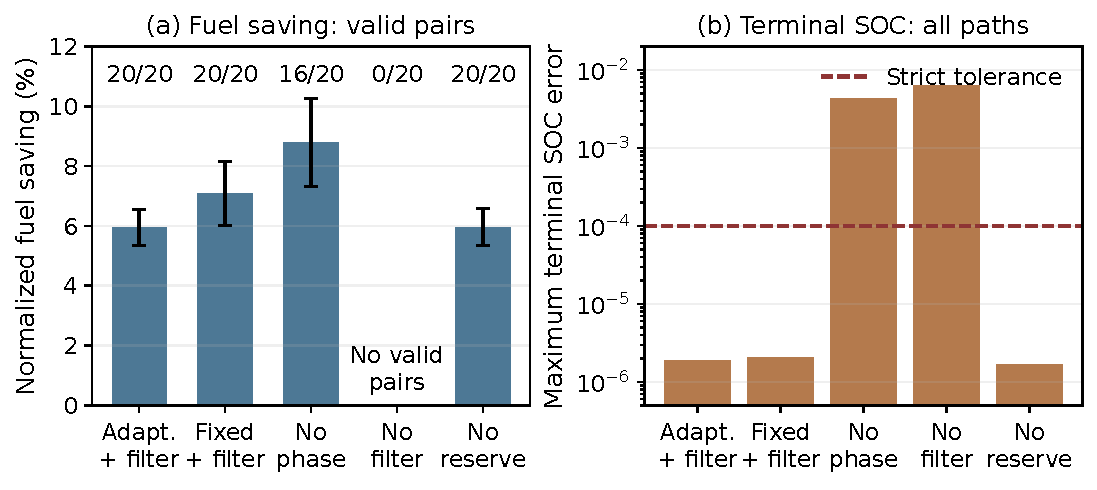
\includegraphics[width=\linewidth]{figures/revision_ablation.pdf}
\caption{Module attribution on the independent set. The~left panel explicitly reports the number of valid pairs; the right panel uses every completed trajectory and the same strict tolerance. Error bars: 95\% Student-t confidence intervals. A~missing saving bar means no valid pair, not zero~saving.}\label{fig:ablation}

\end{figure}

Equal-budget development selects $\lambda=1$ for conventional fixed ECMS and $(\lambda_0,K_p)=(1,60)$ for conventional adaptive ECMS. The~former completes all independent paths but has no terminal-valid pairs; the latter has 2/20 valid pairs. Their completed-only normalized diagnostics are 10.337\% and 8.599\%, respectively, and~are not charge-sustaining performance claims. Adding the common phase reference and safeguard to fixed ECMS restores 20/20 validity and gives the same 7.091\% result as the frozen no-adaptation ablation. This stronger comparator rules out attributing the primary adaptive arm's gain to adaptation alone. S5 reports all counts, intervals and the stepwise additions, including their higher apparent fuel reductions before terminal closure is~enforced.

Figure~\ref{fig:trajectory} shows seed 5120, selected by its predeclared identifier rather than by its saving. The~safeguard constrains terminal drift but remains active throughout the task; it is not a final post-processing repair. Soft-empty events are common because the corridor narrows independently of discrete~reachability.
\vspace{-6pt}
\begin{figure}[H]
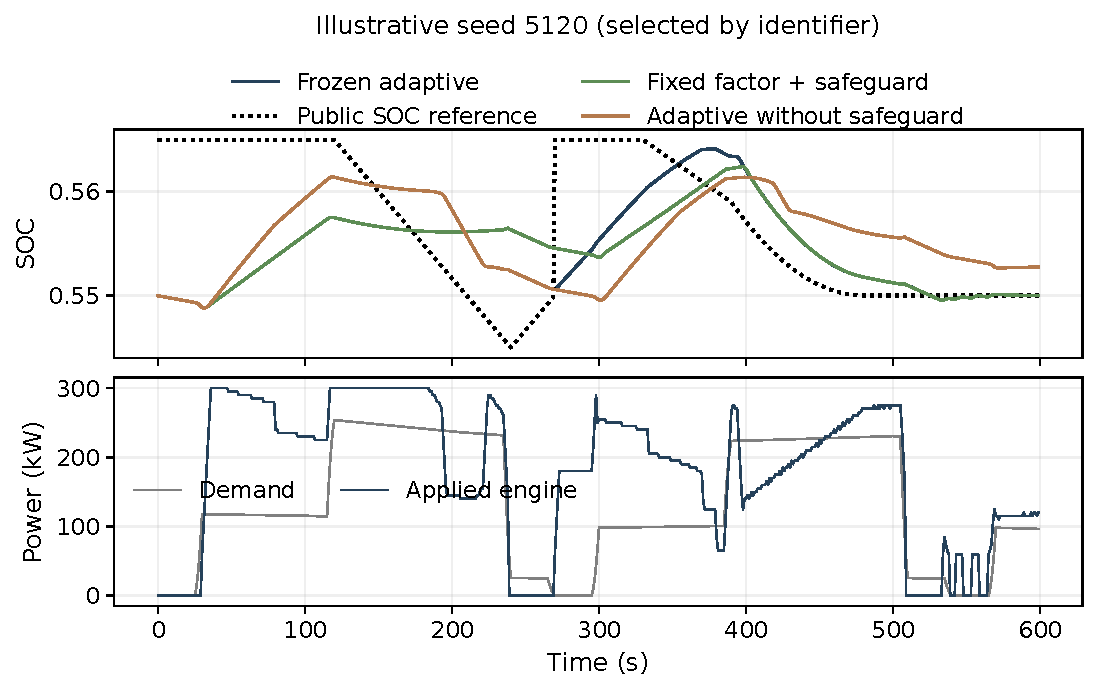
\includegraphics[width=\linewidth]{figures/revision_soc_trajectory.pdf}
\caption{Illustrative current-state trajectories for the first independent seed. Each curve uses its own applied control and the identical input task. The~power panel shows the frozen adaptive arm. The~trajectory is a published result; the public source runner generates a new short diagnostic rather than distributing per-sample data.}\label{fig:trajectory}
\end{figure}
\unskip

\subsection{Same-Parameter Cycle and Component~Sensitivities}
The revised audits all use the submitted $K_p=40$, correcting the previous attribution of $K_p=60$ audits to that frozen configuration. The~deterministic and low-load tasks give 6.604\% and 9.871\% valid-pair saving, respectively. Twenty additional stochastic seeds 5160--5179 all yield valid pairs with mean 6.144\%. The~separate abrupt high-variability task fails for both methods because the current power/ramp-constrained candidate set is empty; no saving is assigned. These are distinct task tests, not repeated physical~measurements. Table~\ref{tab:sensitivity} summarizes the component sensitivities.

\begin{table}[H]
\caption{Independent
 sensitivities with no gain changes ($K_p=40$). Counts distinguish baseline and controller terminal validity; saving uses only their valid intersection. Six-seed grid audits use 5180--5185; map and capacity audits use~5200--5219.}\label{tab:sensitivity}
\small\begin{tabularx}{\linewidth}{@{}Xrrrr@{}}\toprule
\textbf{Audit Input} & \textbf{Baseline Valid} & \textbf{Controller Valid} & \textbf{Valid Pairs} & \textbf{Saving (\%)} \\\midrule
10 kW grid & 6/6 & 6/6 & 6/6 & 6.168 \\
5 kW grid & 6/6 & 6/6 & 6/6 & 6.115 \\
2.5 kW grid & 6/6 & 6/6 & 6/6 & 5.885 \\
Literature-shaped map & 19/20 & 20/20 & 19/20 & 5.724 \\
Low-load map setting 0.15 & 19/20 & 18/20 & 18/20 & 8.011 \\
Low-load map setting 0.25 & 19/20 & 18/20 & 18/20 & 6.509 \\
Low-load map setting 0.35 & 19/20 & 18/20 & 18/20 & 6.086 \\
120 kWh battery & 18/20 & 18/20 & 18/20 & 4.240 \\
200 kWh battery & 19/20 & 20/20 & 19/20 & 5.724 \\
280 kWh battery & 20/20 & 20/20 & 20/20 & 6.204 \\\bottomrule
\end{tabularx}
\end{table}

The three alternative maps each produce one hard failure and one additional completed but SOC-invalid controller path; S6 preserves the reasons and seed identities. The~120~kWh case has two terminal-invalid controller paths, despite completion of all 20. At~200~kWh, the controller is valid on all 20 but the baseline fails terminal closure on one, leaving 19 valid pairs. Fuel averages alone conceal these distinctions. Map/capacity comparisons therefore bound the claim to surviving paired virtual tasks rather than establish universal robustness. The~grid study also shows that exact percentages depend on candidate~discretization.

\subsection{Historical Mechanism and Full-Information~Diagnostics}
The historical legacy fixed-factor ECMS gave 10.491\% direct-fuel saving on a steep-island map but a 0.251\% fuel increase on the literature-shaped map. Legacy terminal-set MPC remained fuel-inferior in both cases. These are separate implementation/map mechanism observations retained in S7; they are not alternative headline values for the revised primary~controller.

The historical favorable full-information diagnostic yields 21.611\% raw and 19.828\% terminal-energy-normalized fuel reduction, i.e.,~approximately 20\%. It uses the complete nominal-task future, a~deliberately steep map, 150 kW electrical limits and a $\pm0.01$ terminal SOC band, whereas the primary online study uses 180 kW and $10^{-4}$. The~literature-shaped oracle attempt failed continuous terminal-SOC replay. A~former 24.087\% grid value also failed replay and is excluded. S7 retains the favorable diagnostic and its battery-energy adjustment explicitly; the value is neither a realizable online saving nor a proven global upper~bound.

\section{Discussion}
\unskip
\subsection{What the Added Evidence~Supports}
The independent experiment supports a positive fuel reduction and strict terminal closure for the frozen adaptive configuration relative to the declared load-following baseline. The~module comparisons narrow its interpretation. The~same safeguard with a fixed factor saves more fuel, while the adaptive factor reduces proposal corrections. The~current results therefore support a fuel--charge--intervention trade-off, not the superiority of adaptive ECMS over conventional ECMS. The~role of the phase reference is also conditional: deleting it permits more terminal failures, while its removal can improve fuel use on surviving pairs. Such outcomes cannot be represented by additive percentages assigned to independent~modules.

The hard constraints, phase reference and terminal accounting distinguish the applied system from an unconstrained instantaneous fuel optimum. Conversely, intervention counts are not a direct wear metric; their importance must be assessed along with starts, actual operating-point changes and a future hardware model. The~fixed-factor arm remains a serious alternative when fuel alone is prioritized within this virtual task. We keep both arms rather than choose the best held-out result after seeing~it.

\subsection{Model Dependence and Feasibility~Limits}
Algebraic conservation does not establish external validity. The~battery capacity is large for a 600 s task, the~steady engine map is rescaled, and~the machine map lacks speed--torque dependence. These assumptions can enlarge or shrink the opportunity for load shifting. The~sensitivity family exposes that dependence, but~does not replace empirical characterization or demonstrate that the electrical, thermal and packaging assumptions can be realized together on a tractor. Hence, the~virtual percentages should not be multiplied by real fuel-use statistics to predict economic or emissions~benefits.

The safeguard enforces only present hard constraints and a soft successor-SOC preference. Unknown future demand, finite candidate resolution, cold-start availability and minimum dwell can make the next hard set empty. A~zero-width terminal corridor can also be unreachable. A~recursive-feasibility result would require an explicitly bounded disturbance set, an~appropriate reachable/invariant construction and a feasible backup policy under the modeled hybrid transitions. None is supplied here, and~we remove the corresponding guarantee language. A~reported 20/20 terminal-valid set is evidence for those paths, not for all~tasks.

\subsection{Practical Implementation and Remaining Evidence~Gaps}
A physical implementation would require measured SOC and current, component operating envelopes including torque and thermal limits, a~calibrated engine conversion map, drivetrain transients and controller-interface latency. Task duration and phase may be uncertain or change during operation; the current corridor assumes they are supplied correctly and does not replan unknown task boundaries. Start fuel and dwell are prescribed, not identified. The~model also omits inverter switching losses, cooling demand variation, battery aging, clutch transitions, turbocharger lag and traction-slip~dynamics.

The finite action search is computationally simple, but~local Python timing is an implementation diagnostic affected by the host and scheduler. It is not embedded deadline certification. The~hard-empty branch currently stops the simulated task; a real controller would require a separately verified reduced-load or safe-state policy. The~absence of physical measurements is appropriate to the theoretical scope, but~necessarily limits deployment and field-economy claims. The~next theoretical extensions are disturbance-bounded reachability, torque-dependent machine envelopes, task-boundary uncertainty and joint parameter perturbations. Hardware validation would answer a different, later~question.

\section{Conclusions}
A phase-informed ECMS with an internal soft SOC safeguard was evaluated in a declared ideal power-split tractor model. The~frozen adaptive configuration reproduces the submitted 5.676\% result and gives 5.951\% normalized saving with 20/20 strict-valid pairs on an independent set. Ablation shows that the SOC safeguard is important for terminal closure in this experiment, whereas adaptation reduces interventions while sacrificing fuel saving relative to fixed ECMS with the same safeguard (7.091\%). Same-gain audits retain positive valid-pair savings but expose terminal failures and hard-action demand boundaries. The~approximately 20\% favorable full-information diagnostic remains explicitly separate. These findings quantify conditional virtual-model trade-offs; they do not prove recursive feasibility, establish adaptive-ECMS fuel superiority or predict measured tractor fuel~economy.

\vspace{+6pt}

\supplementary{The following supporting information can be downloaded at:
 \linksupplementary{s1}, Supplementary Methods and Results S1--S7; full parameter and seed ledgers, development candidates, per-path revision results, model-consistency checks and reproduction code are provided as supporting information for this article.}


\authorcontributions{Conceptualization, C.C.; Methodology, C.C.; Software, C.C.; Formal analysis, C.C.; Visualization, C.C.; Writing---original draft preparation, C.C.; Resources, C.C.; Validation, P.W.; Investigation, C.C.; Writing---review and editing, Y.Z.; Supervision, Y.Z.; Project administration, Y.Z.; Funding acquisition, Y.Z. All authors have read and agreed to the published version of the manuscript.
}
\funding{This work has received funding from the Science and Technology Project of the Ministry of Agriculture and Rural Affairs of~China.}
\institutionalreview{Not applicable.}
\informedconsent{Not applicable.}
\dataavailability{The clean virtual-prototype source code, parameter manifests and minimal source-only reproduction runners are available at
 \url{https://github.com/Fat-pig-Cui/agricultural-tractor-virtual-prototypes} (accessed on 26 October 2026), indexed by Zenodo concept DOI \href{https://doi.org/10.5281/zenodo.22754509}{10.5281/zenodo.22754509}. The~public repository intentionally excludes frozen numerical outputs, per-sample trajectories, checkpoints, review correspondence and submission archives; a fresh run writes newly generated diagnostics to an external workspace.}
\conflictsofinterest{The authors declare no conflicts of~interest.}

\begin{adjustwidth}{-\extralength}{0cm}

\reftitle{References}

\begin{thebibliography}{999}
\bibitem{mousazadeh2011} Mousazadeh, H.; Keyhani, A.; Javadi, A.; Mobli, H.; Abrinia, K.; Sharifi, A. Life-cycle assessment of a Solar Assist Plug-in Hybrid electric Tractor (SAPHT) in comparison with a conventional tractor. \emph{Energy Convers. Manag.} \textbf{2011}, \emph{52}, 1700--1710. \url{https://doi.org/10.1016/j.enconman.2010.10.033}.

\bibitem{mocera2020} Mocera, F.; Som\`a, A. Analysis of a parallel hybrid electric tractor for agricultural applications. \emph{Energies} \textbf{2020}, \emph{13}, 3055. \url{https://doi.org/10.3390/en13123055}.

\bibitem{curiel2023} Curiel-Olivares, G.; Johnson, S.; Escobar, G.; Schacht-Rodr\'iguez, R. Model predictive control-based energy management system for a hybrid electric agricultural tractor. \emph{IEEE Access} \textbf{2023}, \emph{11}, 118801--118811. \url{https://doi.org/10.1109/ACCESS.2023.3322462}.

\bibitem{jilek2008} J\'ilek, L.; Pra\v{z}an, R.; Podp\v{e}ra, V.; Gerndtov\'a, I. The effect of the tractor engine rated power on diesel fuel consumption during material transport. \emph{Res. Agric. Eng.} \textbf{2008}, \emph{54}, 1--8. \url{https://doi.org/10.17221/710-RAE}.

\bibitem{janulevicius2010} Janulevi\v{c}ius, A.; Juostas, A.; Pupinis, G. Tractor engine load and fuel consumption in road construction works. \emph{Transport} \textbf{2010}, \emph{25}, 403--410. \url{https://doi.org/10.3846/transport.2010.50}.

\bibitem{musardo2005} Musardo, C.; Rizzoni, G.; Staccia, B. A-ECMS: An adaptive algorithm for hybrid electric vehicle energy management. {In Proceedings of the 44th IEEE Conference on Decision and Control}, Seville, Spain, 12--15 December 2005; pp. 1816--1823. \url{https://doi.org/10.1109/CDC.2005.1582424}.

\bibitem{sargent2013} Sargent, R.G. Verification and validation of simulation models. \emph{J. Simul.} \textbf{2013}, \emph{7}, 12--24. \url{https://doi.org/10.1057/jos.2012.20}.

\bibitem{mocera2020b} Mocera, F. A model-based design approach for a parallel hybrid electric tractor energy management strategy using hardware in the loop technique. \emph{Vehicles} \textbf{2020}, \emph{3}, 1--19. \url{https://doi.org/10.3390/vehicles3010001}.

\bibitem{wu2024} Wu, Z.; Chen, X.; Liu, S.; Li, Z. An Improved Deep Reinforcement Learning Based Energy Management Strategy for Hybrid Electric Agricultural Tractor. In Proceedings of the {2024 6th International Conference on Power and Energy Technology (ICPET)}, Beijing, China, 12–15 July 2024;

 pp. 1368--1373. \url{https://doi.org/10.1109/ICPET62369.2024.10940675}.

\bibitem{zhao2024} Zhao, S.; Gao, Z.; Li, X.; Li, Y.; Xu, L. Research on Energy Management Strategy of Fuel Cell Tractor Hybrid Power System. \emph{World Electr. Veh. J.} \textbf{2024}, \emph{15}, 61. \url{https://doi.org/10.3390/wevj15020061}.

\bibitem{zhang2024freq} Zhang, M.; Li, X.; Han, D.; Shang, L.; Xu, L. Energy management strategy for fuel cell hybrid tractor considering demand power frequency characteristic compensation. \emph{Sci. Rep.} \textbf{2024}, \emph{14}, 27844. \url{https://doi.org/10.1038/s41598-024-78832-2}.

\bibitem{zhang2024osecvt} Zhang, K.; Deng, X.; Lu, Z.; Wang, T. Research on the energy management strategy of a hybrid tractor OS-ECVT based on a dynamic programming algorithm. \emph{Agriculture} \textbf{2024}, \emph{14}, 1658. \url{https://doi.org/10.3390/agriculture14091658}.

\bibitem{yan2024series} Yan, X.; Zhao, Y.; Liu, X.; Liu, M.; Wu, Y.; Zhang, J. Research on energy management strategy for series hybrid tractor under typical operating conditions based on dynamic programming. \emph{World Electr. Veh. J.} \textbf{2024}, \emph{15}, 156. \url{https://doi.org/10.3390/wevj15040156}.

\bibitem{perez2024} Perez Estevez, M.A.; Melendez Frigola, J.; Armengol Llobet, J.; Alberti, L.; Renzi, M. Optimal design of a series hybrid powertrain for an agricultural tractor. \emph{Energy Convers. Manag. X} \textbf{2024}, \emph{24}, 100789. \url{https://doi.org/10.1016/j.ecmx.2024.100789}.

\bibitem{xie2016} Xie, S.; Sun, F.; He, H.; Peng, J. Plug-in hybrid electric bus energy management based on dynamic programming. \emph{Energy Procedia} \textbf{2016}, \emph{104}, 378--383. \url{https://doi.org/10.1016/j.egypro.2016.12.064}.

\bibitem{ripaccioli2010} Ripaccioli, G.; Bernardini, D.; Di Cairano, S.; Bemporad, A.; Kolmanovsky, I.V. A stochastic model predictive control approach for series hybrid electric vehicle power management. In Proceedings of the 2010 American Control Conference, Baltimore, MD, USA, 30 June--2 July 2010; pp. 5844--5849. \url{https://doi.org/10.1109/ACC.2010.5530504}.


\bibitem{zhang2017} Zhang, S.; Xiong, R.; Sun, F. Model predictive control for power management in a plug-in hybrid electric vehicle with a hybrid energy storage system. \emph{Appl. Energy} \textbf{2017}, \emph{185}, 1654--1662. \url{https://doi.org/10.1016/j.apenergy.2015.12.035}.

\bibitem{wang2016} Wang, H.; Huang, Y.; Khajepour, A.; Song, Q. Model predictive control-based energy management strategy for a series hybrid electric tracked vehicle. \emph{Appl. Energy} \textbf{2016}, \emph{182}, 105--114. \url{https://doi.org/10.1016/j.apenergy.2016.08.085}.

\bibitem{wang2025sizing} Wang, X.; Yao, S.; Li, P.; Chen, Y.; Hao, Q.; Huang, S.; Zhao, Y. Optimal sizing of fuel cell hybrid electric heavy-duty tractor with minimum of unit mileage cost. \emph{Energy Convers. Manag.} \textbf{2025}, \emph{330}, 119674. \url{https://doi.org/10.1016/j.enconman.2025.119674}.

\bibitem{huo2018} Huo, Y.; Yan, F. A predictive energy management strategy for hybrid electric powertrain with a turbocharged diesel engine. \emph{J. Dyn. Syst. Meas. Control} \textbf{2018}, \emph{140}, 061017. \url{https://doi.org/10.1115/1.4039216}.

\bibitem{plett2004} Plett, G.L. Extended Kalman filtering for battery management systems of LiPB-based HEV battery packs. \emph{J. Power Sources} \textbf{2004}, \emph{134}, 252--261. \url{https://doi.org/10.1016/j.jpowsour.2004.02.031}.

\bibitem{wabersich2021} Wabersich, K.P.; Zeilinger, M.N. A predictive safety filter for learning-based control of constrained nonlinear dynamical systems. \emph{Automatica} \textbf{2021}, \emph{129}, 109597. \url{https://doi.org/10.1016/j.automatica.2021.109597}.

\bibitem{devyanin2023} Devyanin, S.N.; Bizhaev, A.V.; Pavlov, Y.D.; Vetrova, S.M.; Barchukova, A.S. Parametric characterization of a tractor engine by specific fuel consumption. \emph{Agric. Mach. Technol.} \textbf{2023}, \emph{17}, 68--74. \url{https://doi.org/10.22314/2073-7599-2023-17-4-68-74}.
\end{thebibliography}
\PublishersNote{}
\end{adjustwidth}
\end{document}
